\documentclass[UTF8]{ctexart}

%固定图片位置
\usepackage{float}

%插入超链接
\usepackage{url}

\usepackage{tikz,mathpazo}
\usetikzlibrary{shapes.geometric, arrows}
\usetikzlibrary{calc}

%\usepackage[affil-it]{authblk}

\usepackage{listings}
%插入代码的配置
\definecolor{CPPLight}  {HTML} {686868}
\definecolor{CPPSteel}  {HTML} {888888}
\definecolor{CPPDark}   {HTML} {262626}
\definecolor{CPPBlue}   {HTML} {4172A3}
\definecolor{CPPGreen}  {HTML} {487818}
\definecolor{CPPBrown}  {HTML} {A07040}
\definecolor{CPPRed}    {HTML} {AD4D3A}
\definecolor{CPPViolet} {HTML} {7040A0}
\definecolor{CPPGray}  {HTML} {B8B8B8}
\lstset{
	language=Matlab,                                     % 设置语言
    columns=fixed,    
    breaklines = true,   
    basicstyle=\small ,
    numbers=left,                                        % 在左侧显示行号
    %frame=none,                                          % 不显示背景边框
    backgroundcolor=\color[RGB]{245,245,244},            % 设定背景颜色
    keywordstyle=\color[RGB]{40,40,255}\bfseries,                 % 设定关键字颜色
    %commentstyle=\color{red!10!green!70}\textit,    % 设置代码注释的颜色
    numberstyle=\tiny\color{darkgray},           % 设定行号格式
    commentstyle=\it\color[RGB]{0,96,96},                % 设置代码注释的格式
    stringstyle=\rmfamily\slshape\color[RGB]{128,0,0},   % 设置字符串格式
    showstringspaces=false,                              % 不显示字符串中的空格                           
    %morekeywords={True,alignas,continute,friend,register,true,alignof,decltype,goto,
    %reinterpret_cast,try,asm,defult,if,return,typedef,auto,delete,inline,short,
    %typeid,bool,do,int,signed,typename,break,double,long,sizeof,union,case,
    %dynamic_cast,mutable,static,unsigned,catch,else,namespace,static_assert,using,
    %char,enum,new,static_cast,virtual,char16_t,char32_t,explict,noexcept,struct,
    %void,export,nullptr,switch,volatile,class,extern,operator,template,wchar_t,
    %const,false,private,this,while,constexpr,float,protected,thread_local,
    %const_cast,for,public,throw,std,rand},
    emph={access,and,break,class,continue,def,del,elif ,else,%
	except,exec,finally,for,from,global,if,import,in,i s,%
	lambda,not,or,pass,print,raise,return,try,while, imshow, subplot, figure,%
    log, fft2, fftshift, abs, size, rgb2gray, imread},
    emphstyle=\color{CPPViolet}\bfseries, 
    emph={[2]True, False, None, self},
	emphstyle=[2]\color{green},
	emph={[3]from, import, as},
	emphstyle=[3]\color{blue},
	upquote=true,
	morecomment=[s]{"""}{"""},
    morecomment=[s]{\%}{},
	%commentstyle=\color{orange}\slshape,
    commentstyle=\color{red!10!green!70}\textit,    % 设置代码注释的颜色
	emph={[4]1, 2, 3, 4, 5, 6, 7, 8, 9, 0},
	emphstyle=[4]\color{red},
	emph={[5]numpy, np, plt},
	emphstyle=[5]\color{red},
	literate=*{:}{{\textcolor{blue}:}}{1}%
	{=}{{\textcolor{blue}=}}{1}%
	{-}{{\textcolor{blue}-}}{1}%
	{+}{{\textcolor{blue}+}}{1}%
	{*}{{\textcolor{blue}*}}{1}%
	{!}{{\textcolor{blue}!}}{1}%
	{(}{{\textcolor{blue}(}}{1}%
	{)}{{\textcolor{blue})}}{1}%
	{[}{{\textcolor{blue}[}}{1}%
	{]}{{\textcolor{blue}]}}{1}%
	{<}{{\textcolor{blue}<}}{1}%
	{>}{{\textcolor{blue}>}}{1},%
    %{\%}{{\textcolor{green}\%}}{1},%
	framexleftmargin=0.1mm, framextopmargin=0.1mm, frame=shadowbox, rulesepcolor=\color{black},
}



\usepackage{geometry}
\geometry{left=1.2cm, right=1.2cm, top=1.2cm, bottom=1.2cm}

%得到引用的标题内容
\usepackage{nameref} 

%添加首行缩进,两个字符
\usepackage{indentfirst}
\setlength{\parindent}{2em}

%多行公式一个编号
\usepackage{amsmath}

%文献引用,标准类型为plain
%\usepackage[hyperref=true,backend=biber,sorting=none,backref=true]{biblatex}
%\addbibresource{ref.bib}
\bibliographystyle{plain}
\usepackage{cite}

\pagestyle{plain}

%跨页表格
\usepackage{multirow}
\usepackage{longtable,booktabs}
\usepackage{supertabular}
\usepackage{makecell}

%调整itemize等的间距
\usepackage{enumitem}


\usepackage{graphicx}
\usepackage{subfigure}

%超链接
\usepackage[linkcolor=yellow,citecolor=red,backref=page,hyperfootnotes=true]{hyperref}
\hypersetup{
bookmarks=true,
colorlinks=true,
linkcolor=black
}
\usepackage{tabularx} %This package must be placed after package {hyperref}, otherwise footnote marks are NOT treated as hyperlinks.


%引入了一些改进的数学环境,如align
\usepackage{amsmath}

\title{数字图像处理实验报告四}
\author{姓名:鲁国锐 \protect\newline
\and 学号:17020021031 \\
\and 专业:电子信息科学与技术}
%\date{2020年4月22日}

\begin{document}
	\maketitle
	\renewcommand{\contentsname}{目录}
	\renewcommand{\listfigurename}{插图目录}
	\renewcommand{\listtablename}{表格目录}
	\renewcommand{\refname}{参考文献}
	\renewcommand{\abstractname}{摘要}
	\renewcommand{\indexname}{索引}
	\renewcommand{\tablename}{表}
	\renewcommand{\figurename}{图}
	
	
	
	\tableofcontents
	\newpage
	
	\hypersetup{
	bookmarks=true,
	colorlinks=true,
	linkcolor=red,
	urlcolor=blue
	}
    
    \section{实验目标}
    
                \begin{enumerate}[leftmargin=50pt]
    				\item 熟悉图像复原的各种方法;
    				\item 复习并实现各种相关滤波器(巴特沃斯、高斯等);
    				\item 利用滤波器去除周期性噪声;
    				\item 学习并使用自适应滤波器。
    			\end{enumerate}    

	\section{实验一}
	\indent $Test$ 目录下有图像$windmill\_noise.png$,用$Matlab$写程序,去除条纹干扰。

			
%			\begin{figure}[H]
%				\centering 
%				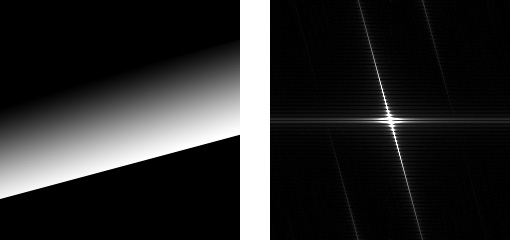
\includegraphics[scale=0.4]{org_img.png} 
%				\caption{原图及其傅里叶变换} 
%				\label{problem_img}
%			\end{figure}
%		
%        
        \subsection{思路}
            \indent 参考\cite{邹园园2009基于频域滤波的}的思路:
    			
                \begin{enumerate}[leftmargin=50pt]
    				\item 构建一个类,对原图进行傅里叶变换,并将相关的变量都存进成员变量中;
                    \item 计算沿频谱图行、列方向上的累积分布函数;
                    \item 显示连个累积分布函数,并在图中标出所有波峰和波谷;
                    \item 分别在两幅图中找出离中心波峰最近且相对突出的波峰作为噪声的位置,求出噪声在频谱图中到中心的距离;
                    \item 将求得的距离作为截止频率对原图进行巴特沃斯带阻滤波和高斯带阻滤波器;
                    \item 显示滤波后的图像及其频谱图。
    			\end{enumerate}                
            
         
        \subsection{代码实现}
           
             \begin{lstlisting}[language=Matlab,caption={$remove\_waves$类},label={broadcast.cpp}]
classdef remove_waves < handle
    % 必须加handle,不然不能再构造函数以外的函数里改变成员变量
    properties( SetAccess = public, GetAccess = public )
        im_path; % 完整的路径
        path; % 图像所在目录
        im_name; % 图像文件名
        ext; % 图像扩展名
        im_orig; % 原图
        im_double; % 把原图转换成double
        M; % 行数
        N; % 列数
        F; % 原图的傅里叶变换
        logF; % log(1+abs(F))
        spectrum; % 把F的值映射到0~1范围
        SDv;
        SDu;
        SDv_pk; % SDv的峰值
        SDv_pkloc; % SDv峰值的位置
        SDv_valleyloc; % SDv波谷的位置
        SDu_pk;% SDu的峰值
        SDu_pkloc; % SDu峰值的位置
        SDu_valleyloc; % SDu波谷的位置
    end
    
    methods
        % 构造函数
        function obj = remove_waves(img_path)
            obj.im_path = img_path;
            [obj.path, obj.im_name, obj.ext]  = fileparts(img_path);
            obj.path = strcat(obj.path, '\');
            obj.im_orig = imread(img_path); % 读取图像
            obj.im_double = im2double(obj.im_orig); % 将图像转为double
            [obj.M, obj.N] = size(obj.im_orig); % 得到图像的行数、列数
            % 计算原图的傅里叶变换
            obj.F = fft2(obj.im_double);
            obj.F = fftshift(obj.F);
            % 把频谱图的值映射到0~1范围
            obj.logF = log(1+abs(obj.F));
            obj.spectrum = obj.logF / max(max(obj.logF));
            % 计算累计分布函数
            obj.projection();
            % 显示原图及频谱
            h = figure
            subplot(2, 1, 1), imshow(obj.im_orig), title('原图')
            subplot(2, 1, 2), imshow(obj.spectrum), title('原图频谱图')
            % 使用print函数保存图像,可以保存为更高的分辨率(600)
            print(h, '-dpng', '-r600', strcat(obj.path, 'spectrum_of_img.png'))
        end     
    end
    
    
    
    methods
        % 计算投影图
        function projection(obj)
            % 初始化两个方向的累计函数值
            obj.SDv = zeros(1, obj.N);
            obj.SDu = zeros(1, obj.M);
            % 计算列方向上的累积分布函数
            for v = 1 : obj.N
                for u = 1 : obj.M
                    obj.SDv(v) = obj.SDv(v) + obj.logF(u, v);
                end
            end
            % 找SDv所有峰值及其坐标
            [obj.SDv_pk, obj.SDv_pkloc] = findpeaks(obj.SDv);
            % 取SDu的相反数,可用findpeaks求得所有波谷的坐标
            [temp, obj.SDv_valleyloc] = findpeaks(-obj.SDv);
            % 计算行方向上的累积分布函数
            for u = 1 : obj.M
                for v = 1 : obj.N
                    obj.SDu(u) = obj.SDu(u) + obj.logF(u, v);
                end
            end
            % 找SDu所有峰值及其坐标
            [obj.SDu_pk, obj.SDu_pkloc] = findpeaks(obj.SDu);
            % 取SDu的相反数,可用findpeaks求得所有波谷的坐标
            [temp, obj.SDu_valleyloc] = findpeaks(-obj.SDu);
            
            figure
            % 画出原函数
            subplot(2, 1, 1), plot(obj.SDv), hold on 
            % 标出所有的峰值
            subplot(2, 1, 1), plot(obj.SDv_pkloc, obj.SDv_pk, 'r.', 'Markersize', 2), hold on
            % 标出所有波谷
            subplot(2, 1, 1), plot(obj.SDv_valleyloc, obj.SDv(obj.SDv_valleyloc), 'g.', 'Markersize', 2)
            title('列方向累积分布函数'), xlabel('v'), ylabel('S_D(v)')
            % 画出原函数
            subplot(2, 1, 2), plot(obj.SDu), hold on
            % 标出所有的峰值
            subplot(2, 1, 2), plot(obj.SDu_pkloc, obj.SDu_pk, 'r.', 'Markersize', 2), hold on
            % 标出所有波谷
            subplot(2, 1, 2), plot(obj.SDu_valleyloc, obj.SDu(obj.SDu_valleyloc), 'g.', 'Markersize', 2)
            title('行方向累积分布函数'), xlabel('u'), ylabel('S_D(u)')
            name = strcat(obj.path, 'SD.png');
            %saveas(gcf, strcat(obj.path, 'SD.png'))
            % 可以保存成更高分辨率的图像,-r600设置分辨率
            print(gcf, '-dpng', '-r600', name);
            
        end
    end
            
end

              \end{lstlisting}
    
    \begin{lstlisting}[language=Matlab,caption={$remove\_wave$}]
object = remove_waves(im_path) % 构建remove_waves对象
%找到峰值中心,需要根据具体情况分析出
SDv_pk_cent = floor(length( object.SDv_pk) / 2) + 1; 
% 找出噪声频率距离直流分量在频谱图上的水平距离,需要看图来确定
dx = 5;
v = object.SDv_pkloc(SDv_pk_cent) - object.SDv_pkloc(SDv_pk_cent - dx)
% 找出噪声频率距离直流分量在频谱图上的垂直距离,需要看图来确定
dy = 0;
u = 0
% 计算噪声频率距离频谱中心的距离,及截断频率
D0 = sqrt(v^2 + u^2)
% 找出阻带宽度,需要看图来确定
% 找到波谷中心,需要根据具体情况分析
SDv_valley_cent = length(object.SDv_valleyloc) / 2; 
% 计算阻带宽度
w = object.SDv_valleyloc(SDv_valley_cent-3) - object.SDv_pkloc(SDv_pk_cent - 6)

%% 巴特沃斯滤波
n = 3; % 阶数为3
G = object.F; % 复制一份频谱用作滤波
cent = [ object.M/2+1, object.N/2+1 ] % 确定频谱的中心点坐标
for u = 1 : object.M
    for v = 1 : object.N
        d = sqrt( (u-cent(1))^2 + (v-cent(2))^2); % 当前点到中心点的距离
        % 用巴特沃斯滤波器的公式进行滤波
        G(u, v) = 1 / (1 + (w * d / ( d^2 - D0^2 ))^(2*n)) * G(u, v); 
    end
end
g=real(ifft2(fftshift(G)));% 对滤波后的频谱进行反变换
h = figure % 指定句柄
% 画出滤波后的空间域图像
subplot(2,1,1),imshow(g,[]);
title('巴特沃斯阻带滤波后的图像')
% 在对滤波后的空间域图像进行傅里叶变换,画出滤波后的频谱图
F=fft2(g); 
fc=fftshift(F); 
s=log(1+abs(fc));      
subplot(2,1,2),imshow(s,[]); 
title('巴特沃斯阻带滤波后的频谱图');
print(h, '-dpng', '-r600', strcat(object.path, 'filtered_img.png') )
%% 高斯滤波
G = object.F; % 复制一份频谱用作滤波
for u = 1 : object.M
    for v = 1 : object.N
        d = sqrt( (u-cent(1))^2 + (v-cent(2))^2); % 当前点到中心点的距离
        % 用高斯滤波器的公式进行滤波,1-exp(-1/2*(((d1.^2)-D0^2)./(d1*w)).^2)
        G(u, v) = (1 - exp( -1/2 * ( ( d^2 - D0^2 ) / (d * w) )^2 ) ) * G(u, v); 
    end
end
g=real(ifft2(fftshift(G)));% 对滤波后的频谱进行反变换
h = figure % 指定句柄
% 画出滤波后的空间域图像
subplot(2,1,1),imshow(g,[]);
title('高斯阻带滤波后的图像')
% 在对滤波后的空间域图像进行傅里叶变换,画出滤波后的频谱图
F=fft2(g); 
fc=fftshift(F); 
s=log(1+abs(fc));      
subplot(2,1,2),imshow(s,[]); 
title('高斯阻带滤波后的频谱图');
print(h, '-dpng', '-r600', strcat(object.path, 'Gaussian_filtered_img.png') )
    
                  \end{lstlisting}
        \subsection{结果展示}
        

                        
                        \begin{figure}[H]
                            \centering
                            \subfigure[原图]{
                                \begin{minipage}{0.45\linewidth}
                                    \centering
                                    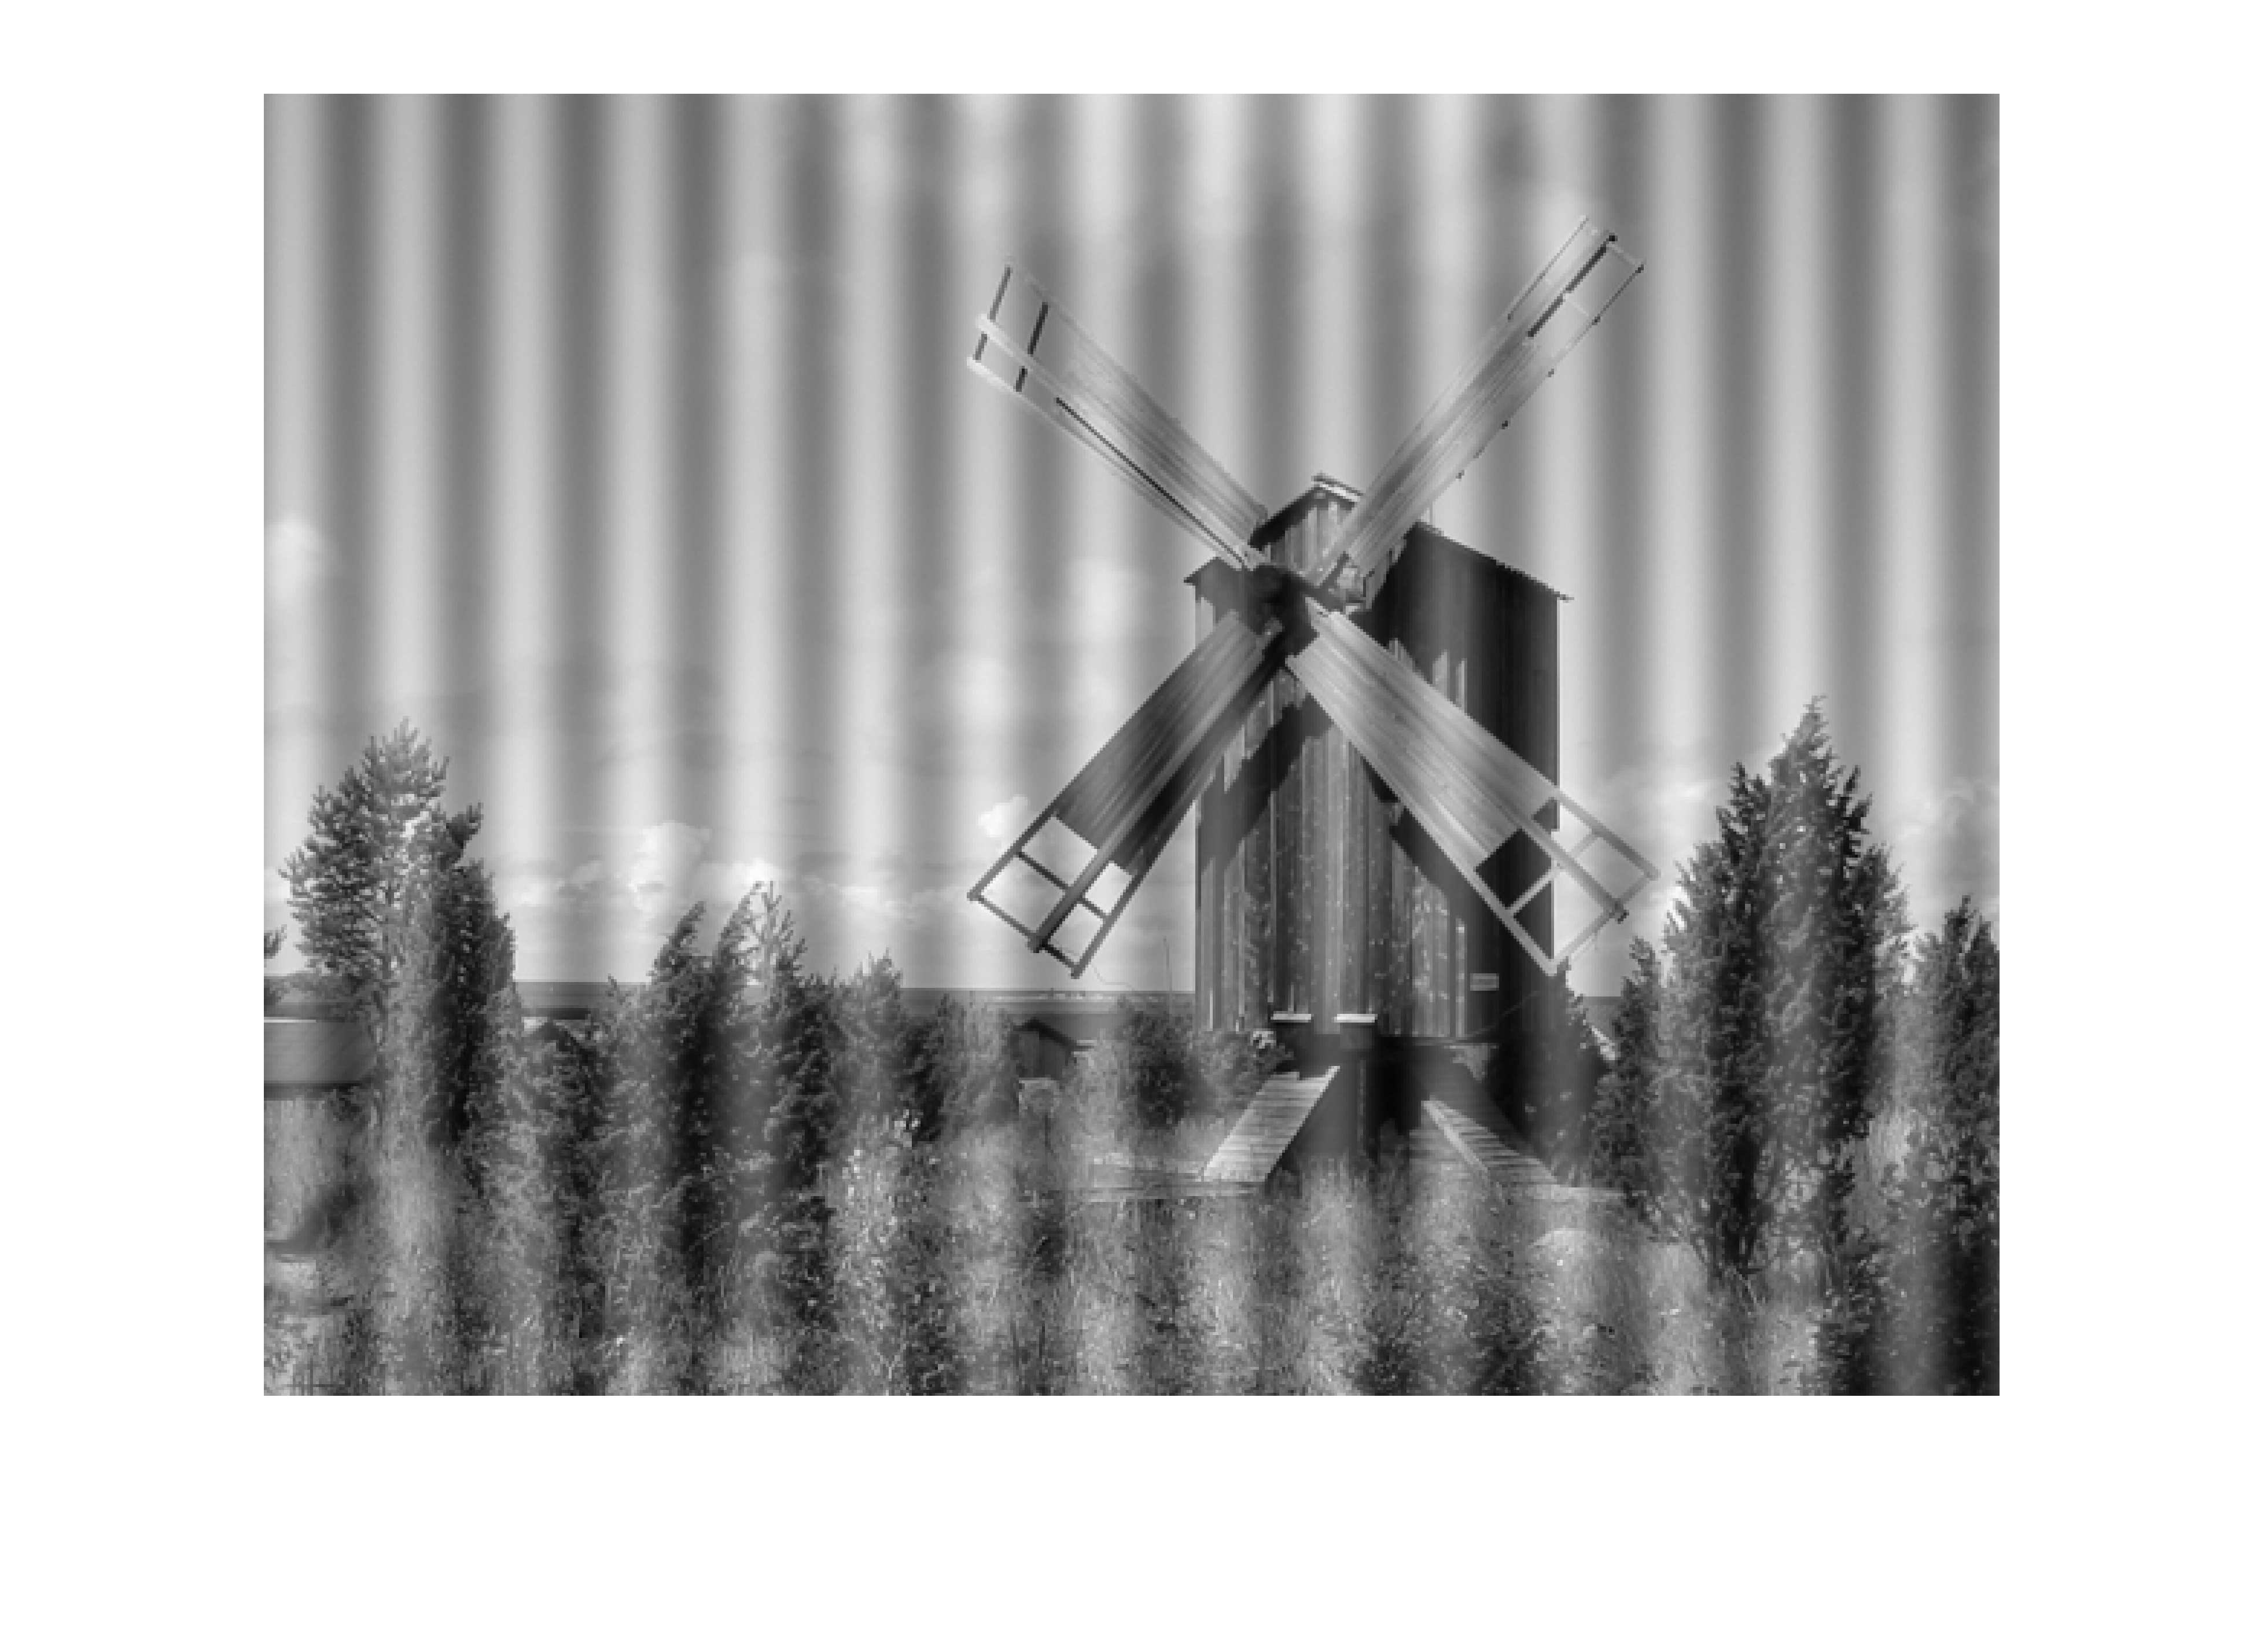
\includegraphics[scale=0.5]{../test/orig_img.png}
                                    %\caption{原图3}
                                \end{minipage}
                            }
                            \subfigure[频谱图]{
                                \begin{minipage}{0.45\linewidth}
                                    \centering
                                    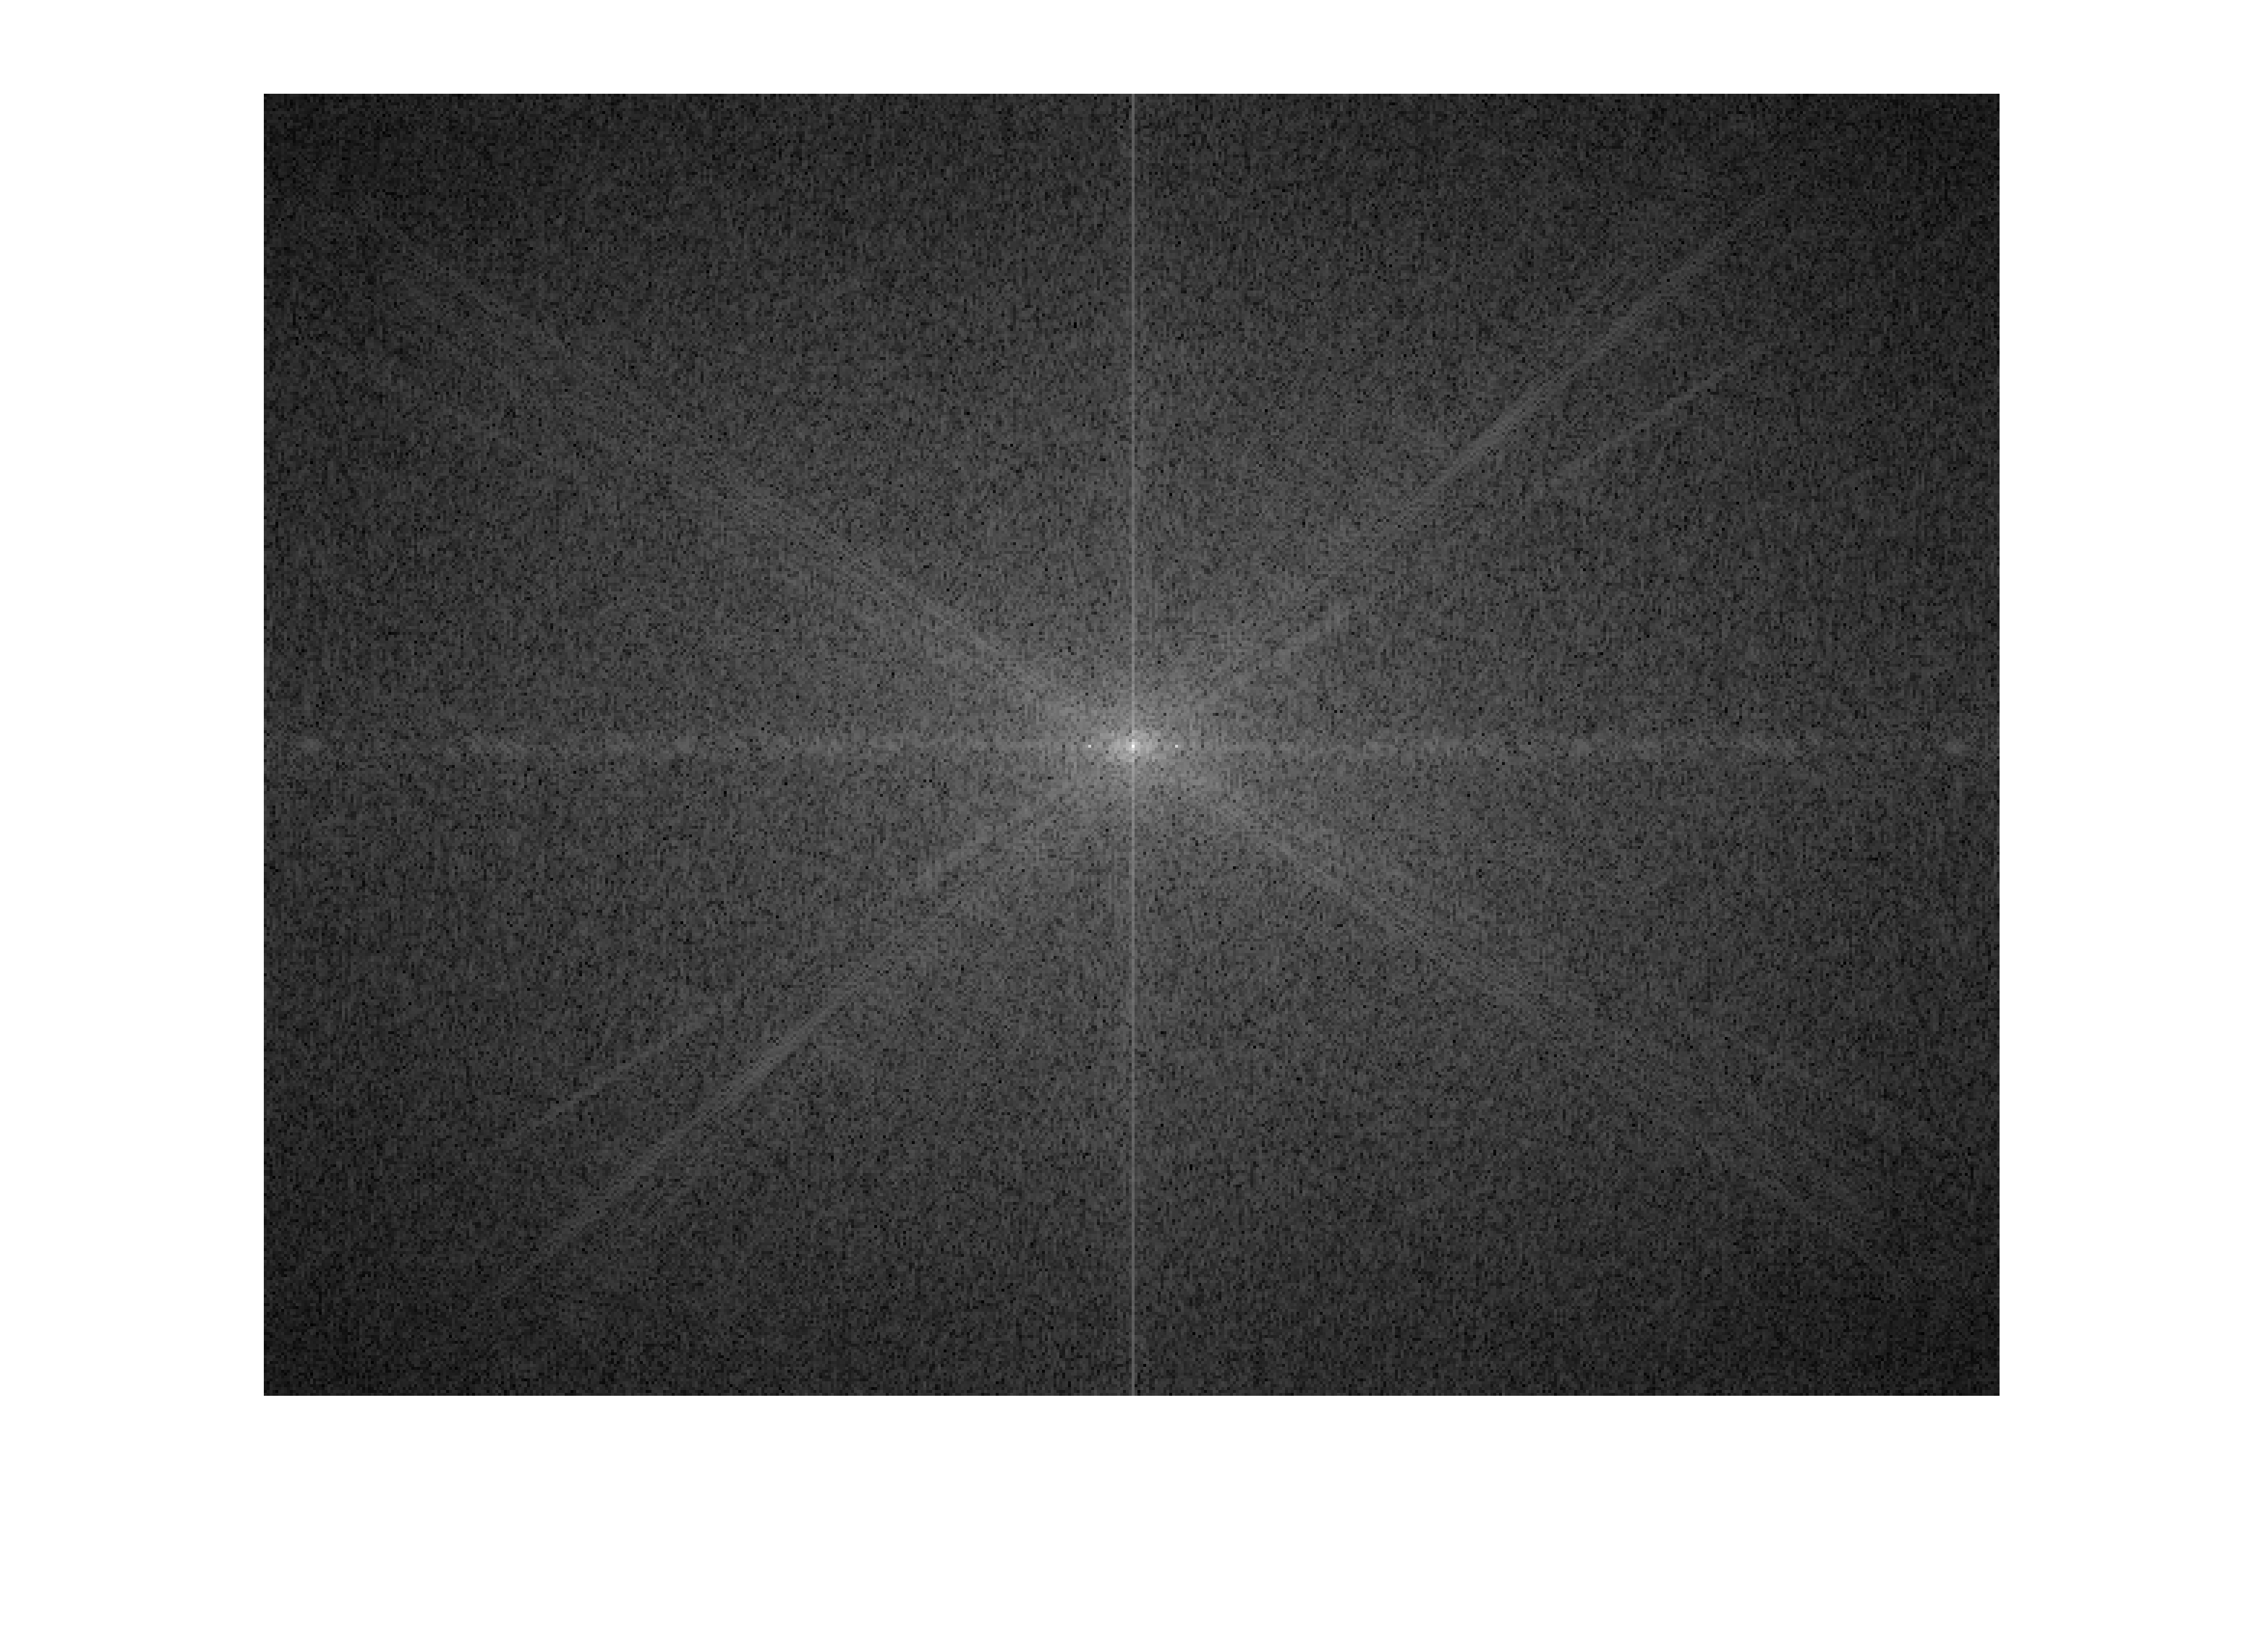
\includegraphics[scale=0.5]{../test/orig_img_spectrum.png}
                                    %\caption{结果3}
                                    \label{res4-4}
                                \end{minipage}
                            }
                            
                            \caption{测试结果}
                            \label{res4}
                        \end{figure}
                        
        
            			\begin{figure}[H]
            				\centering 
            				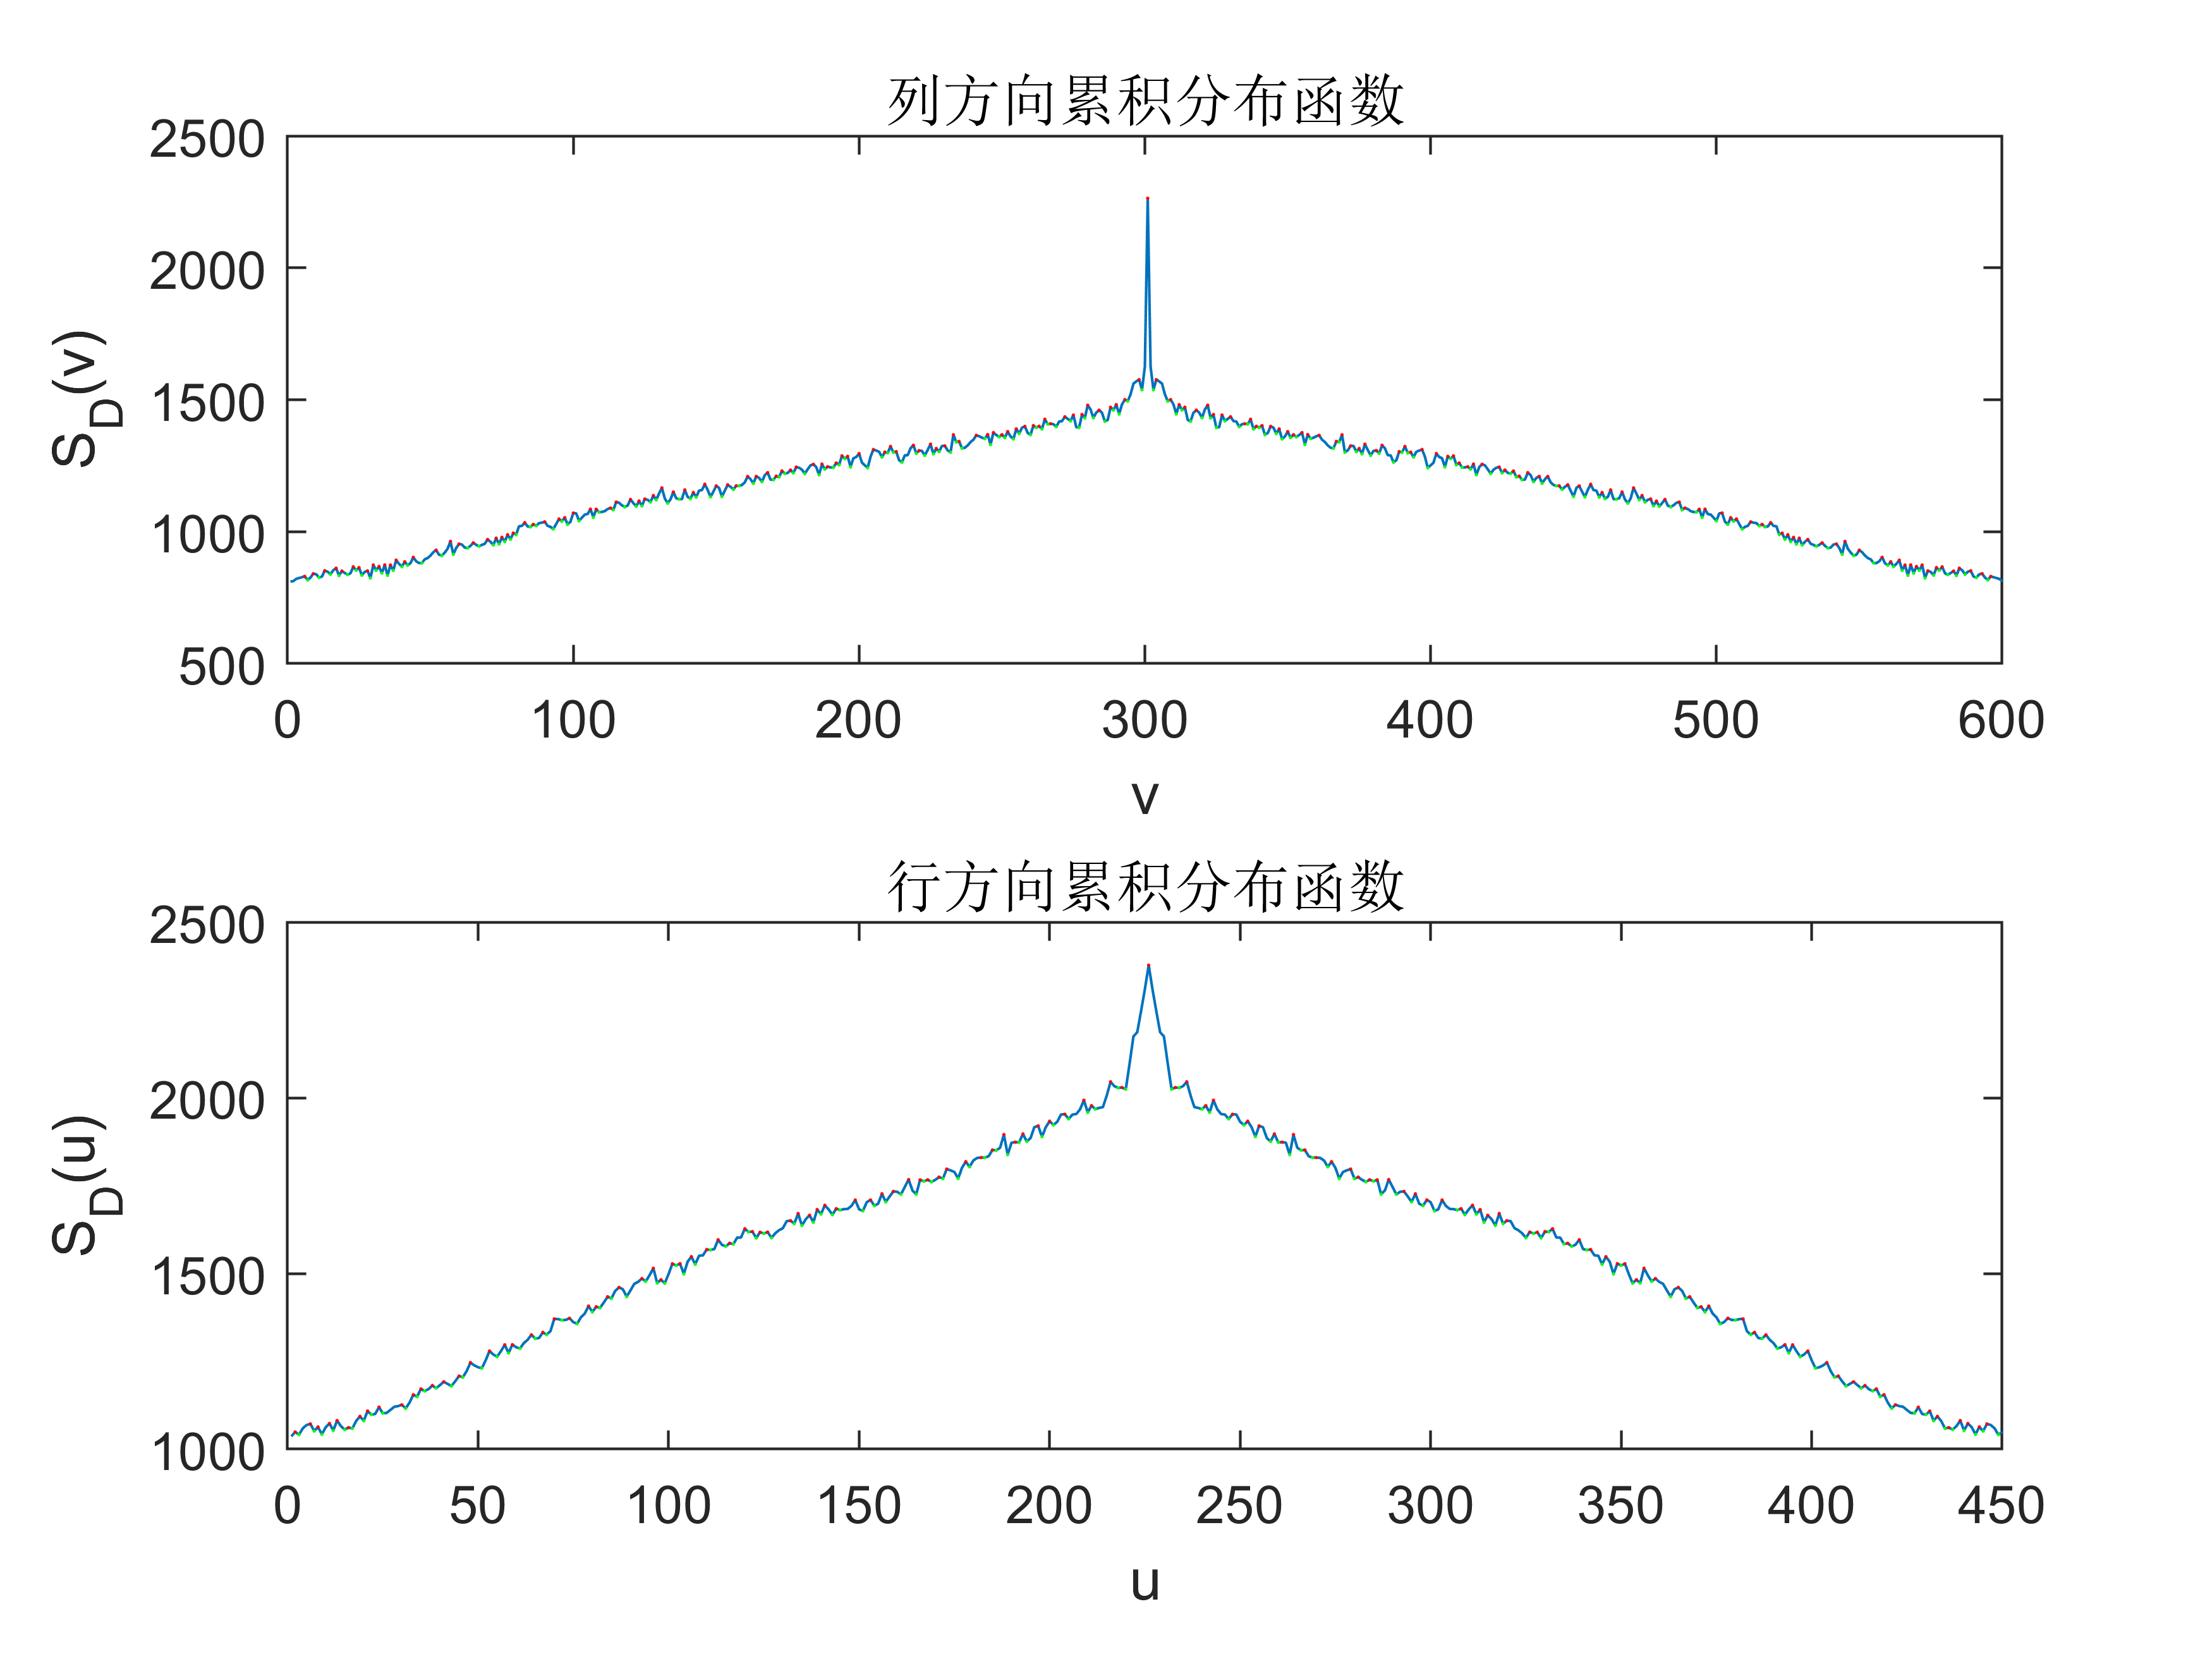
\includegraphics[scale=1]{../test/SD.png} 
            				\caption{累积分布函数} 
            				\label{cumulative_distribution_function}
            			\end{figure}                         

                        \begin{figure}[H]
                            \centering
                            \subfigure[巴特沃斯带阻滤波后的图像]{
                                \begin{minipage}{0.45\linewidth}
                                    \centering
                                    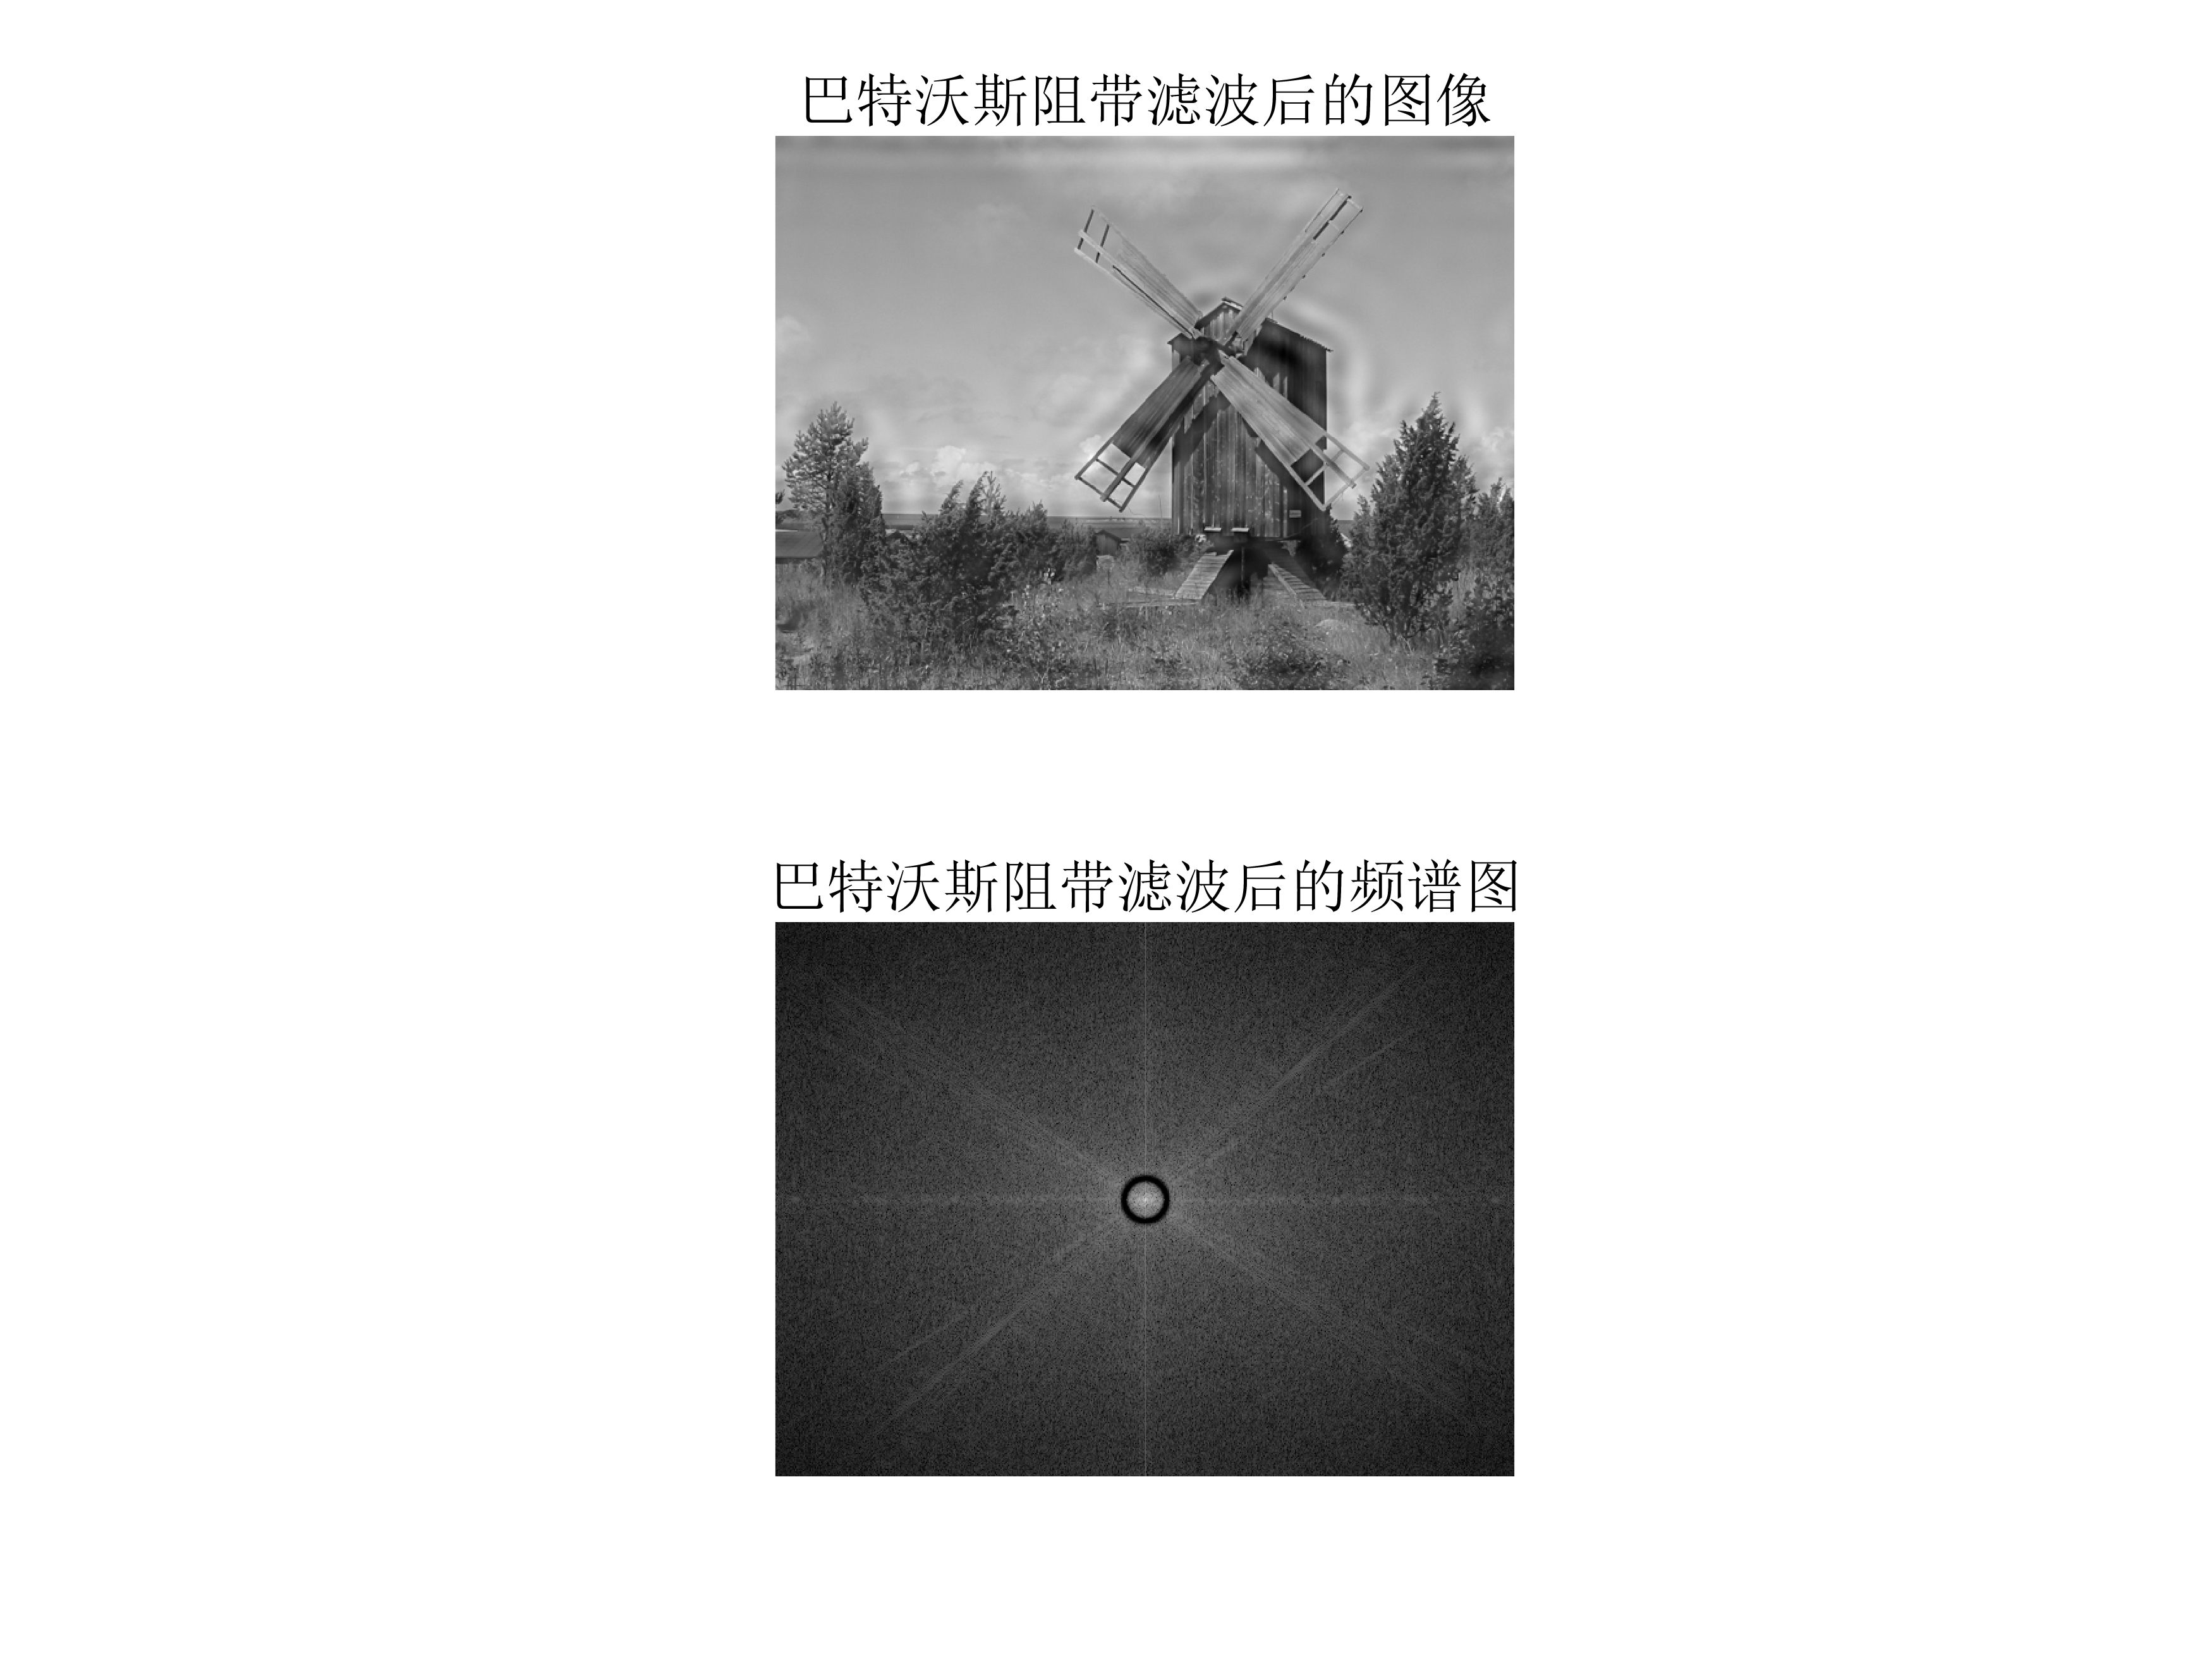
\includegraphics[scale=0.5]{../test/filtered_img.png}
                                    %\caption{原图3}
                                \end{minipage}
                            }
                            \subfigure[巴特沃斯带阻滤波后的频谱图]{
                                \begin{minipage}{0.45\linewidth}
                                    \centering
                                    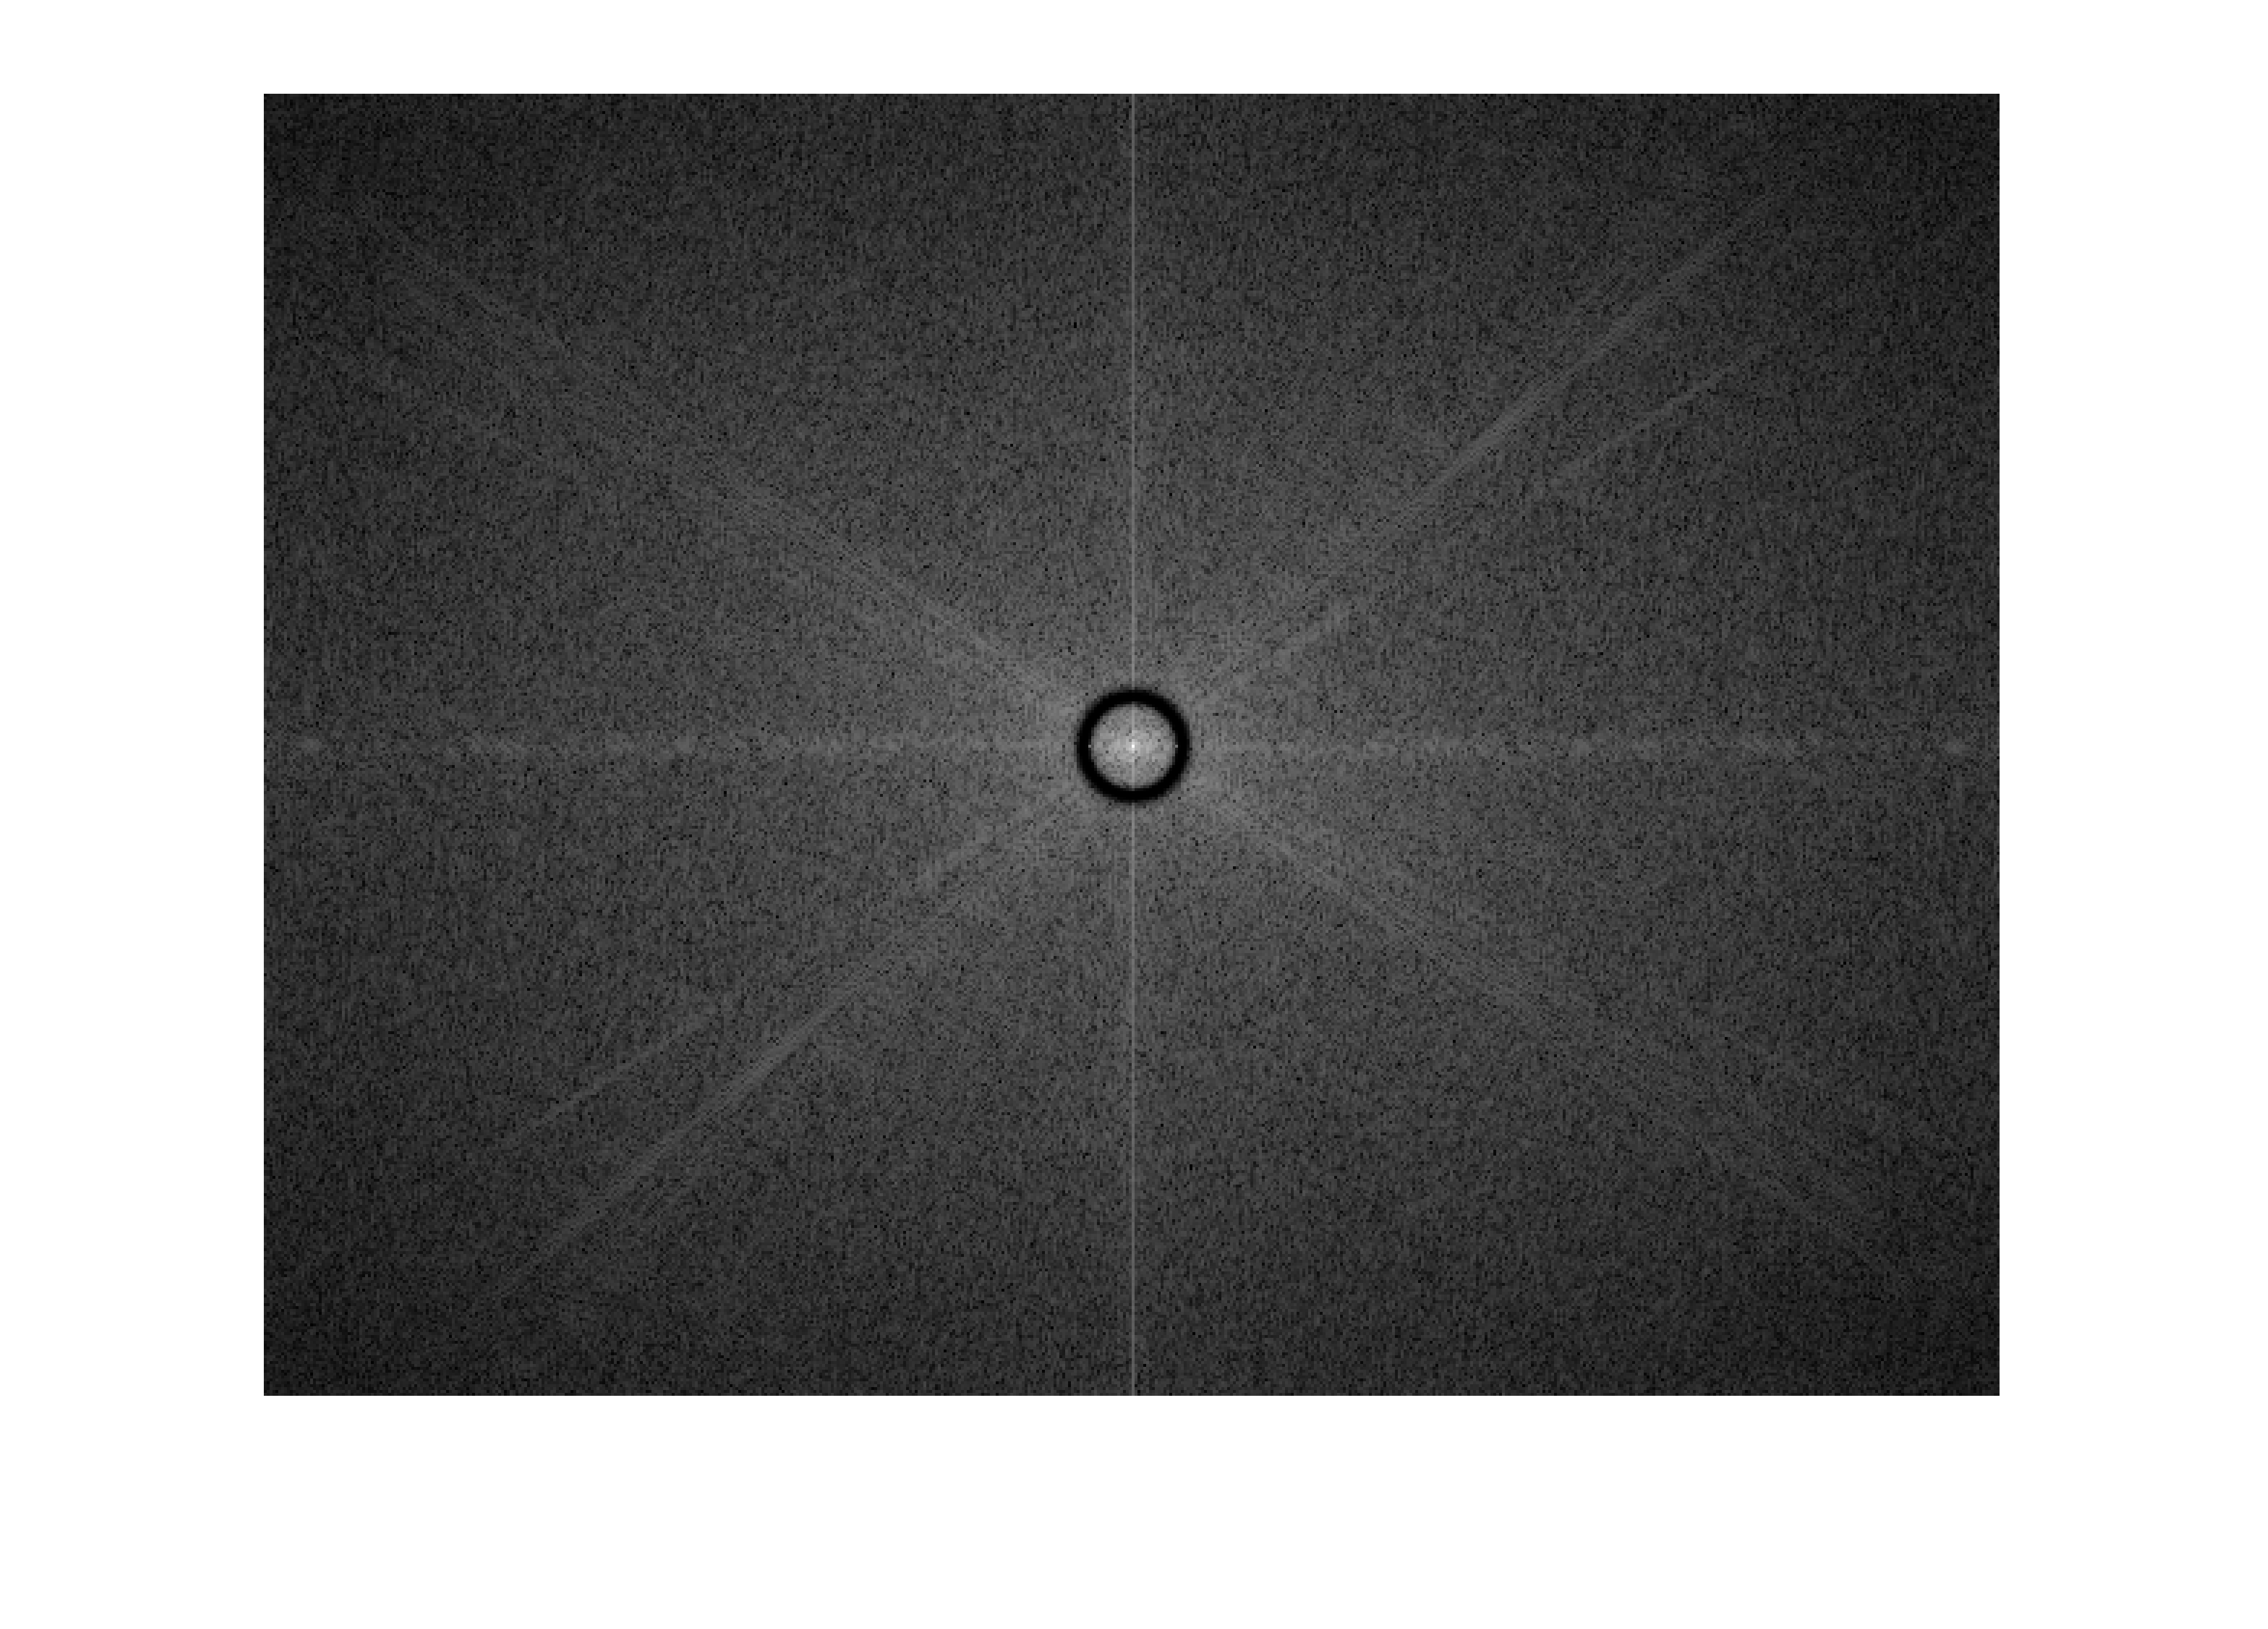
\includegraphics[scale=0.5]{../test/filtered_spectrum.png}
                                    %\caption{结果3}
                                    \label{res4-4}
                                \end{minipage}
                            }
                            
                            \caption{测试结果}
                            \label{butterworth}
                        \end{figure}                        
                      
                        \begin{figure}[H]
                            \centering
                            \subfigure[高斯带阻滤波后的图像]{
                                \begin{minipage}{0.45\linewidth}
                                    \centering
                                    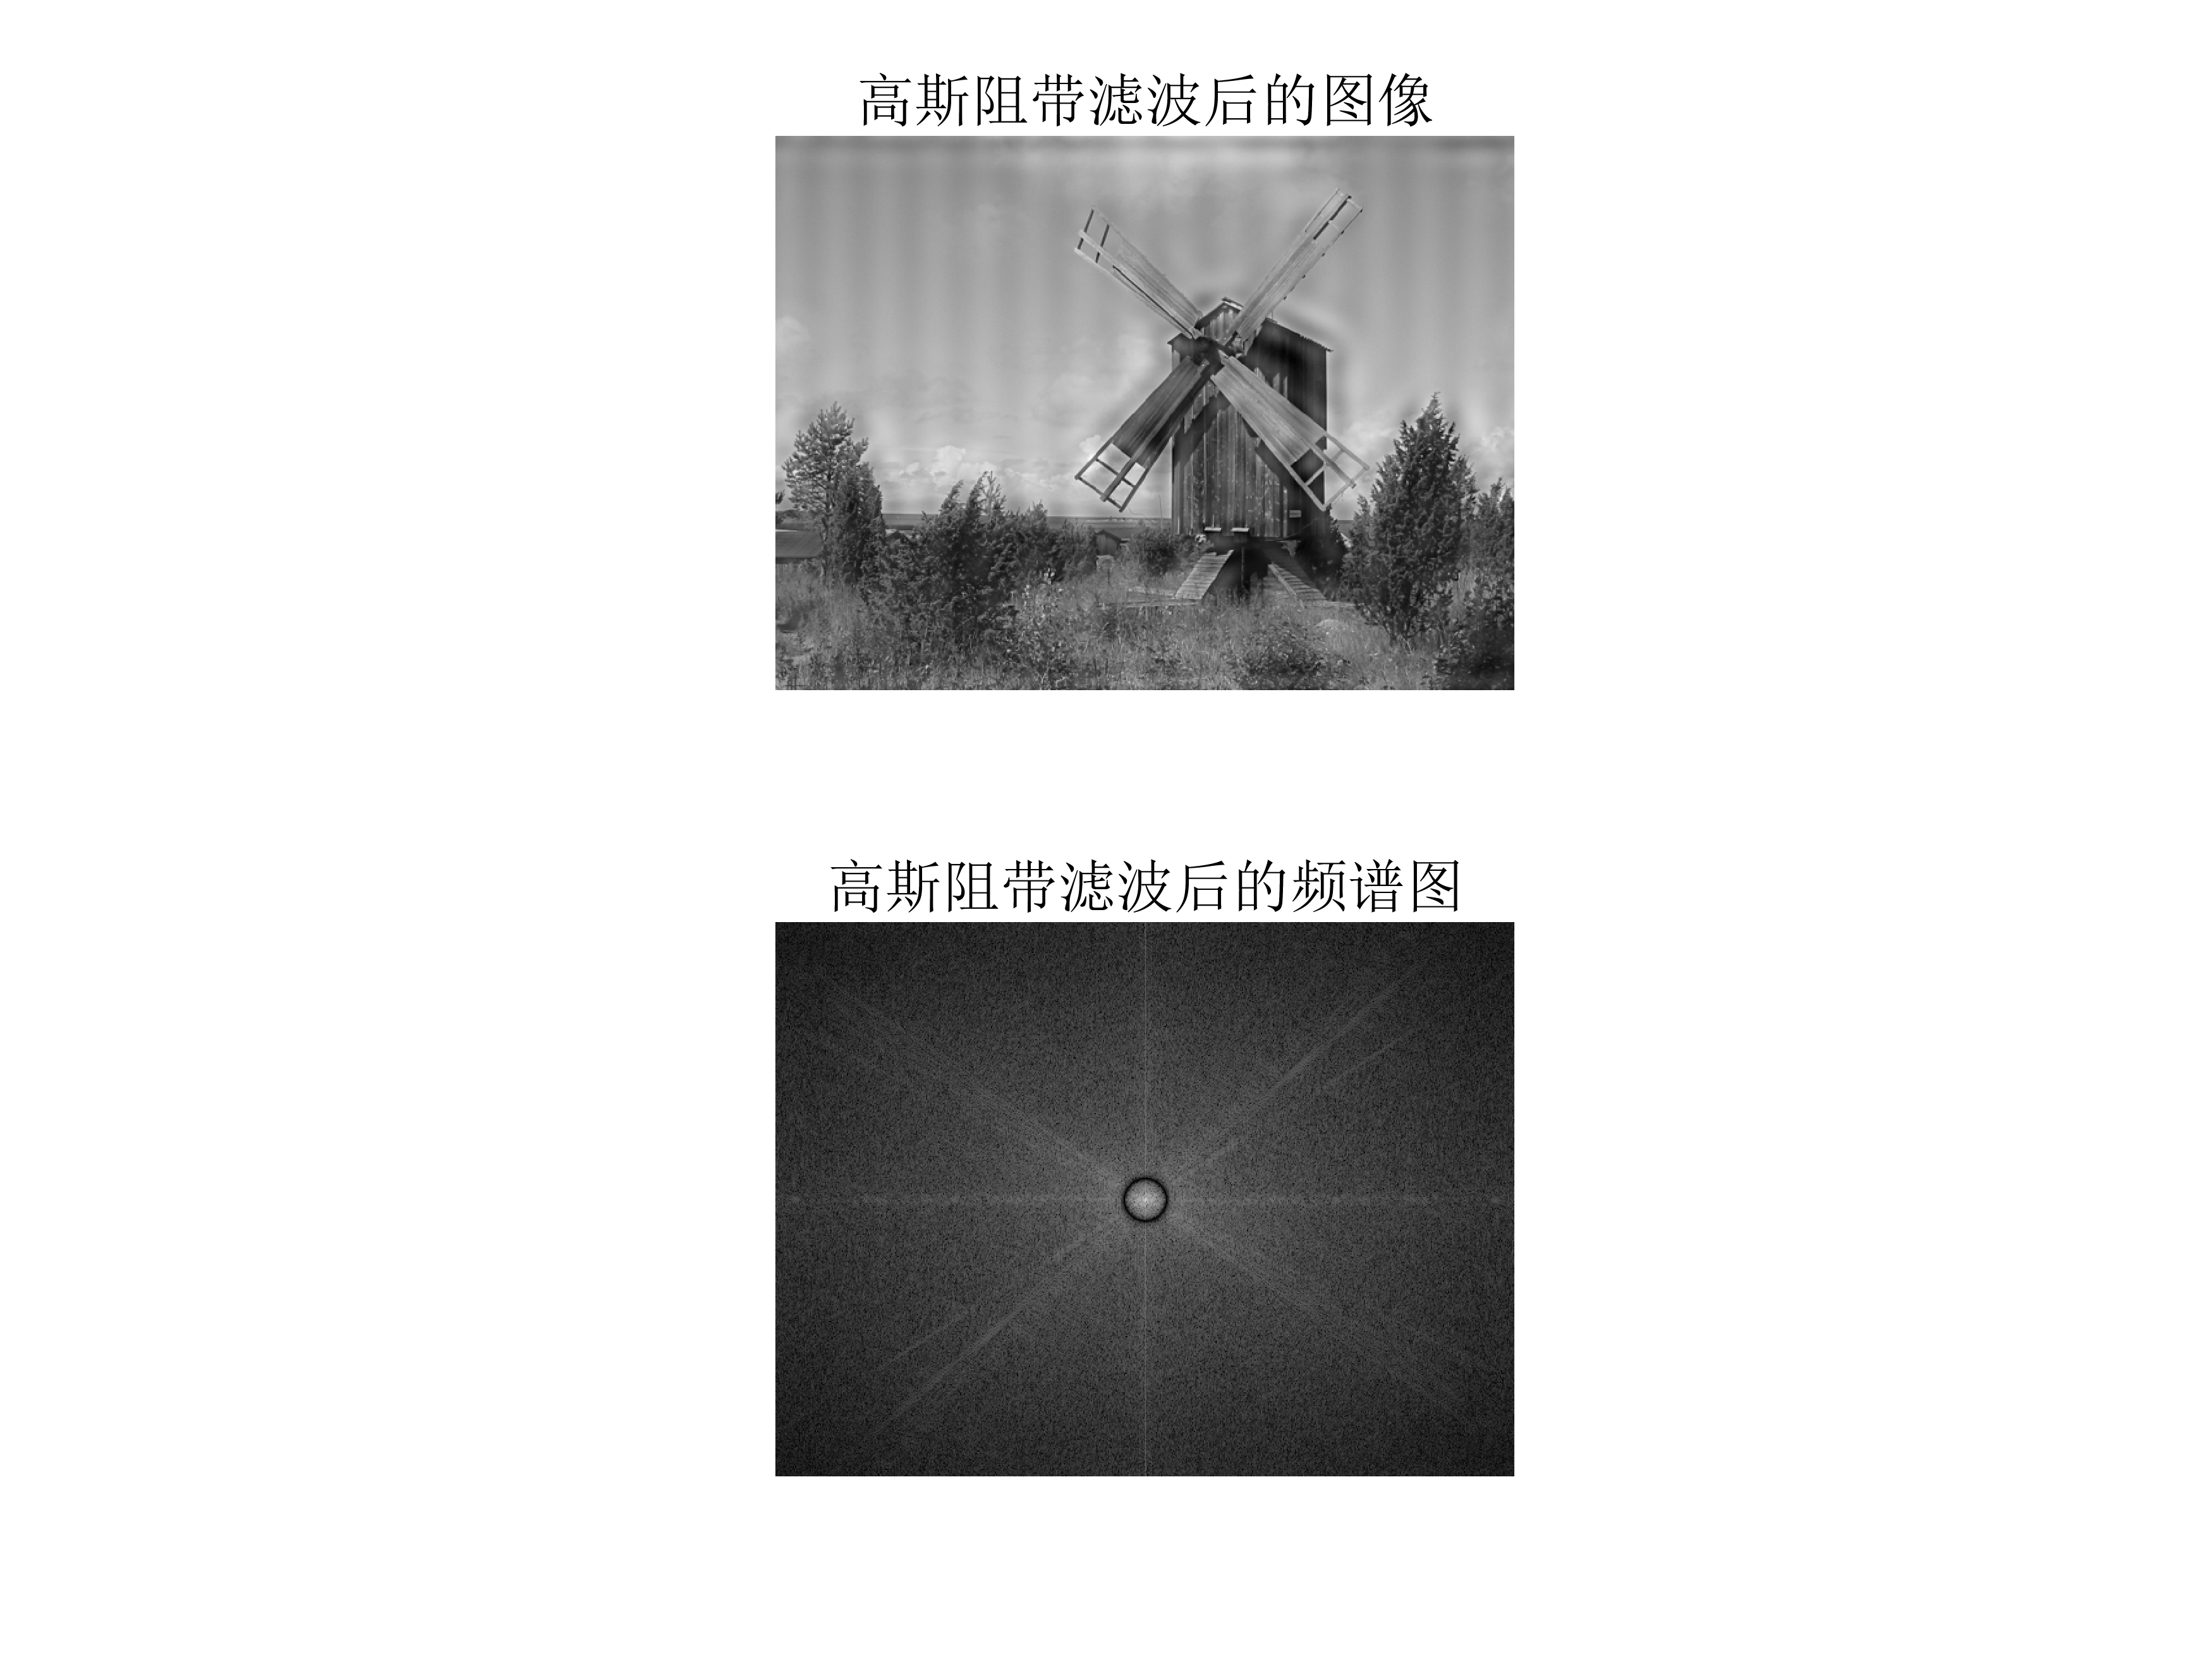
\includegraphics[scale=0.5]{../test/Gaussian_filtered_img.png}
                                    %\caption{原图3}
                                \end{minipage}
                            }
                            \subfigure[高斯带阻滤波后的频谱图]{
                                \begin{minipage}{0.45\linewidth}
                                    \centering
                                    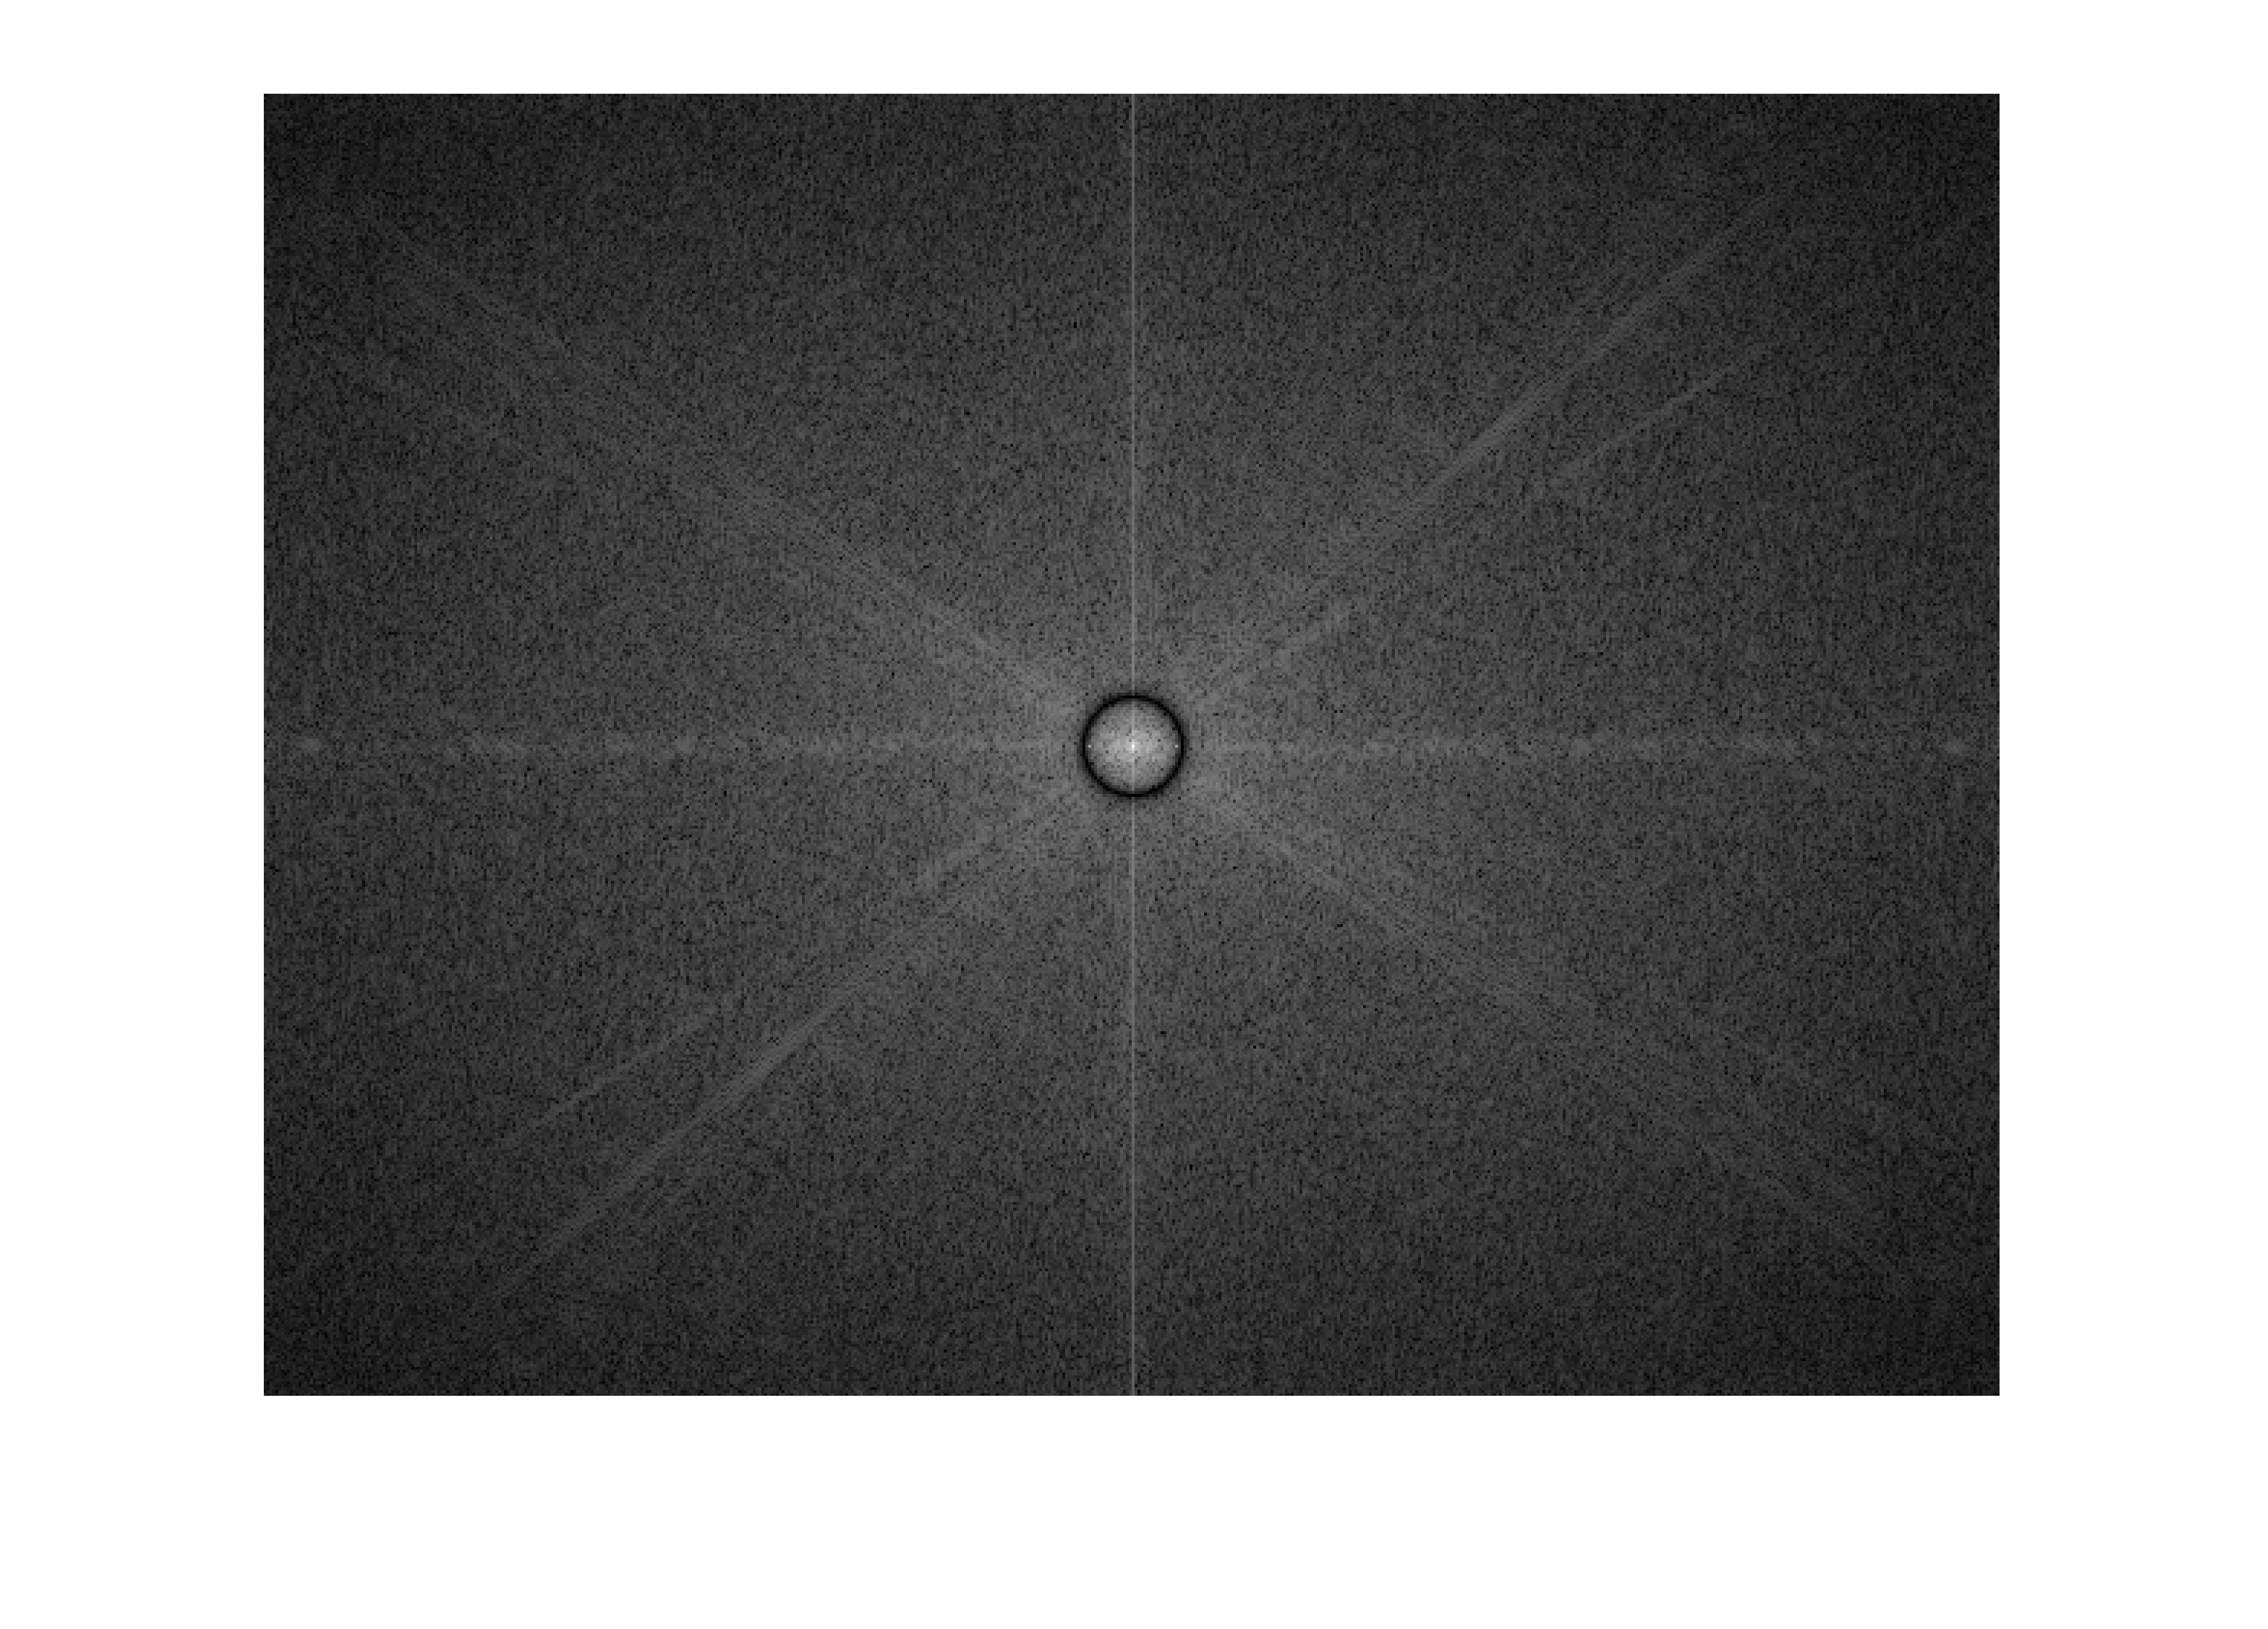
\includegraphics[scale=0.5]{../test/Gaussian_filtered_spectrum.png}
                                    %\caption{结果3}
                                    \label{res4-4}
                                \end{minipage}
                            }
                            
                            \caption{测试结果}
                            \label{gaussian}
                        \end{figure}                              
                        
    
    \section{实验二}
            \indent $Test$目录下有图像$boardWithNoise.jpg$,用$Matlab$写程序,采用自适应中值滤波器去除噪声干扰。
            
        \subsection{思路}
            \indent 参考\cite{齐春亮2005自适应中值滤波器}
         
            
            


	\section{总结}
		\indent 本次实验分为两个部分:第一个部分要求我们用所学的方法去除一副图像中的条纹干扰;第二个部分是要求我们学习并使用滤波器对另一幅图像进行处理。
        
        \indent 第一个部分最大的难点在于如何确定噪声的频率,即准确算出噪声在频谱图中到中心点的距离。关于这一点在实验提供的文献中有一个方案,即分别在行、列方向上计算并画出它的累积分布函数。由于有噪声的存在,在中心峰值的附近应当会有一个相对突出的小波峰。分别在行、列方向的累积分布函数中找到这两个波分的位置,就能确定其行、列坐标。
        
        \indent 理论上这样是可行的,从论文中给的图片来看也确实有用。但在本次实验过程中,待处理图片的噪声在频谱中的能量并不突出,因而导致难以从两个累计分布函数中找到对应的小波峰。
        
        \indent 此外,如何确定小波峰的坐标也是一个问题。这里我所采用的方法是分别对两个累积分布函数使用$findpeaks$函数。该函数可以返回每一个极大值点的值及其坐标。我们用它找到在累计函数分布图中用红点标出所有小波峰,然后对原函数的相反数在用一遍$findpeaks$,便可找出所有小波谷的位置,并在图中用绿点标记出来(如图\ref{cumulative_distribution_function}所示)。之后便需要由人来数出所求小波峰到中心波峰之间的小波峰数目$m$,然后再在$findpeaks$返回的波峰坐标中确定中心波峰的位置,再往前推$m+1$个位置即可求得小波峰在原频谱图中的坐标。波谷的位置可用类似的方法求出。
        
        \indent 按照上述办法求出来的截止频率误差比较大,主要是由于小波峰不突出,难以确定其坐标,所以最后又稍微调了一下参数。得到如图\ref{butterworth}和图\ref{gaussian}所示的结果。可以看出,巴特沃斯带阻滤波的去除效果还不错,而高斯带阻滤波则还有比较明显的噪声残余。
%			\begin{figure}[H]
%				\centering 
%				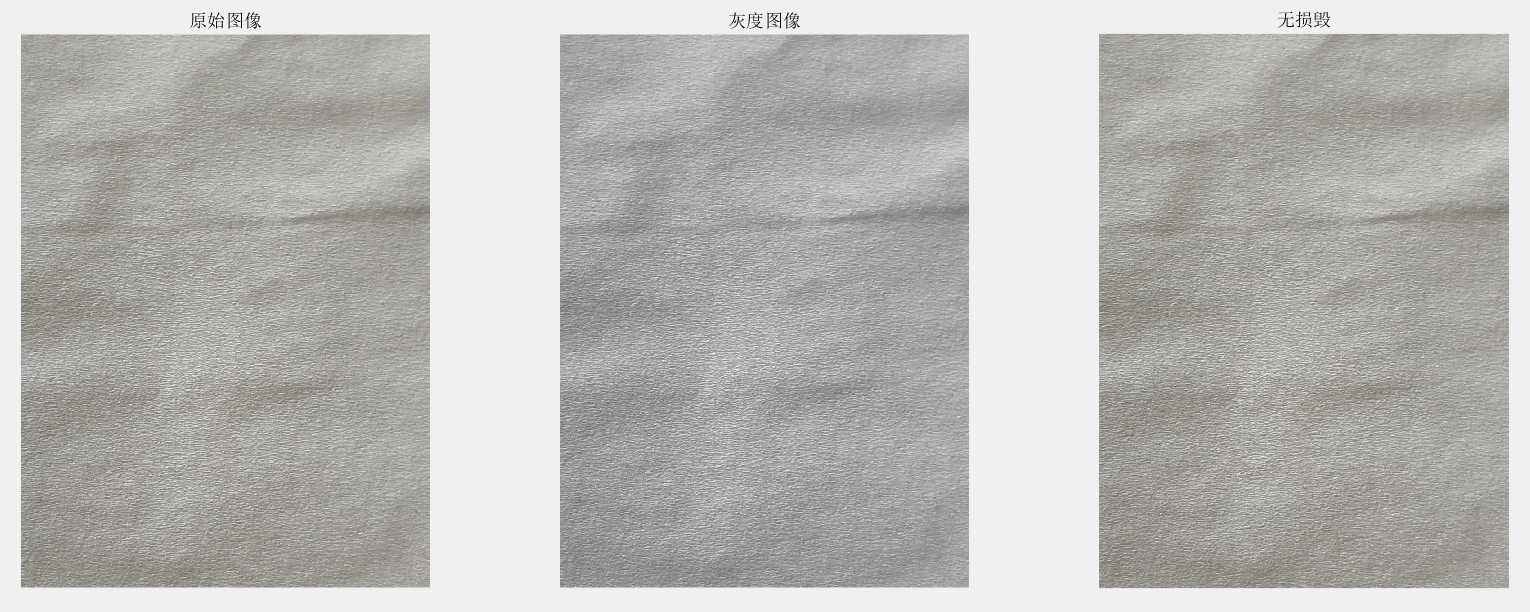
\includegraphics[scale=0.4]{res4.png} 
%				\caption{结果4} 
%				\label{res4}
%			\end{figure}
		

		
%			\begin{figure}[H]
%				\centering 
%				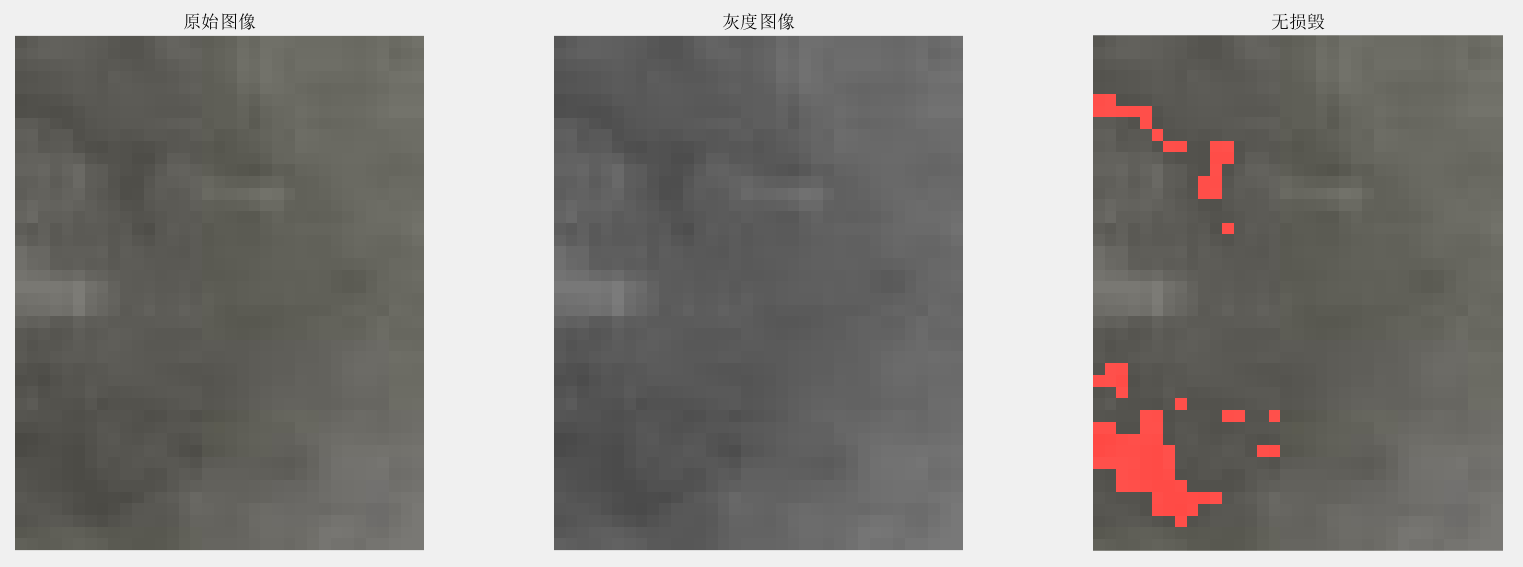
\includegraphics[scale=0.4]{res6.png} 
%				\caption{结果6(截取自结果5的阴影部分)} 
%				\label{res6}
%			\end{figure}
	
	
% 中文文献多个作者用中文逗号“,”连接
%\bibliography{ref.bib}
%\bibliographystyle{abbrv}
\bibliography{ref.bib}


\end{document}